%%%%%%%%%%%%%%%%%%%%%%% file template.tex %%%%%%%%%%%%%%%%%%%%%%%%%
%
% This is a template file for Web of Conferences Journal
%
% Copy it to a new file with a new name and use it as the basis
% for your article
%
%%%%%%%%%%%%%%%%%%%%%%%%%% EDP Science %%%%%%%%%%%%%%%%%%%%%%%%%%%%
%
%%%\documentclass[option]{webofc}
%%% "twocolumn" for typesetting an article in two columns format (default one column)
%
\documentclass{webofc}
\usepackage[varg]{txfonts}   % Web of Conferences font
%
% Put here some packages required or/and some personal commands

\usepackage{xspace}
\usepackage{tabularx}

\newcommand{\pd}{protoDUNE\xspace}
\newcommand{\filesize}{8\,GB\xspace}


%
%
\begin{document}
%
\title{The Prompt Processing System and Data Quality Monitoring in the \pd-SP experiment}
%
%%%\subtitle{Do you have a subtitle?\\ If so, write it here}
\author{ 
\lastname{Maxim Potekhin}\inst{1}\fnsep\thanks{\email{potekhin@bnl.gov}} \it{on behalf of the DUNE Collaboration}
}

\institute{Brookhaven National Laboratory, Upton, NY11973, USA}



\abstract{%
The DUNE Collaboration is conducting an experimental program named ''protoDUNE''
 which includes a beam test of large-scale DUNE prototypes located at CERN in 2018,
and a cosmic ray run in 2019. This paper concerns itself with the single-phase version
of the Liquid Argon Time Projection Chamber which is the principal component of
the detector. Both the volume of the data taken and the sustained rate of data transmittion
to mass storage are quite substantial. In order to support the substantial Data Quality Monitoring
requirements of the experiment we have designed and deployed a Prompt Processing System
 that is complementary to the Online Monitoring and is characterized by a lower bandwidth,
substantial CPU resources and end-to-end latency on the scale of a few minutes and perhaps
tens of minutes. 
}
%
\maketitle
%
\section{Introduction}
\label{sec:intro}
The \pd-SP experiment utilizes a large-scale prototype of the single-phase version of the
Liquid Argon Time Projection Chamber (LArTPC) which will eventually become one
of the principal elements of the DUNE apparatus to be constructed at the Sanford Underground
Research Facility \cite{cdrVol1, cdrVol4}. The prototype (CERN designation NP04) is tested
utilizing a dedicated beam line  at the CERN SPS accelerator complex,
and the run plan also includes a large number of cosmic ray triggers. The layout of the
experimental area is shown in Fig.\,\ref{fig:np02np04}, with the single-phase detector seen as
a cubic structure (the cryostat) on the right-hand side of the diagram. 
In order to provide
the cosmic ray triggering capability an external system of scintillation counters is installed
outside of the cryostat. There is also an array of beam instrumentation devices utilized
in the beam trigger logic and characterization of the beam.

 Located in the vicinity of the detectors
are enclosures for the online computing infrastructure (including Data Acquisition, Online Buffer etc). 
which shown schematically as yellow blocks in the upper-right portion of  the diagram.
There is a dedicated 20 Gb/s network connection to the CERN central storage facilities.
The Data Acquisition System is equipped with an Online Monitor which receives data via the network
and does processing in real time.
Certain types of processing in the category of Data Quality Monitoring (DQM)
require more resources than are available within the DAQ footprint, and include jobs that take substantially
longer time than processes run in the Online Monitor. It is also necessary to insulate DAQ from
potential disruptions due to constant software updates of the DQM software during commissioning
and operation of \pd.
For these reasons a separate ``\pd Prompt Processing System''
(abbreviated as \textbf{p3s}) was put in place \cite{eps} with the following characteristics:
\begin{itemize} 

\item lower bandwidth as compared to the Online Monitor (i.e. a small fraction of events is processed,
but in more detail)

\item extensive and scalable computing resources relying on the CERN batch facility

\item reading data from disk, with no direct coupling to the DAQ system

\item flexibility in introducing, modifying and configuring software without any risk of disruption of
critical DAQ functionality

\end{itemize}

\begin{figure}[tb]
\centering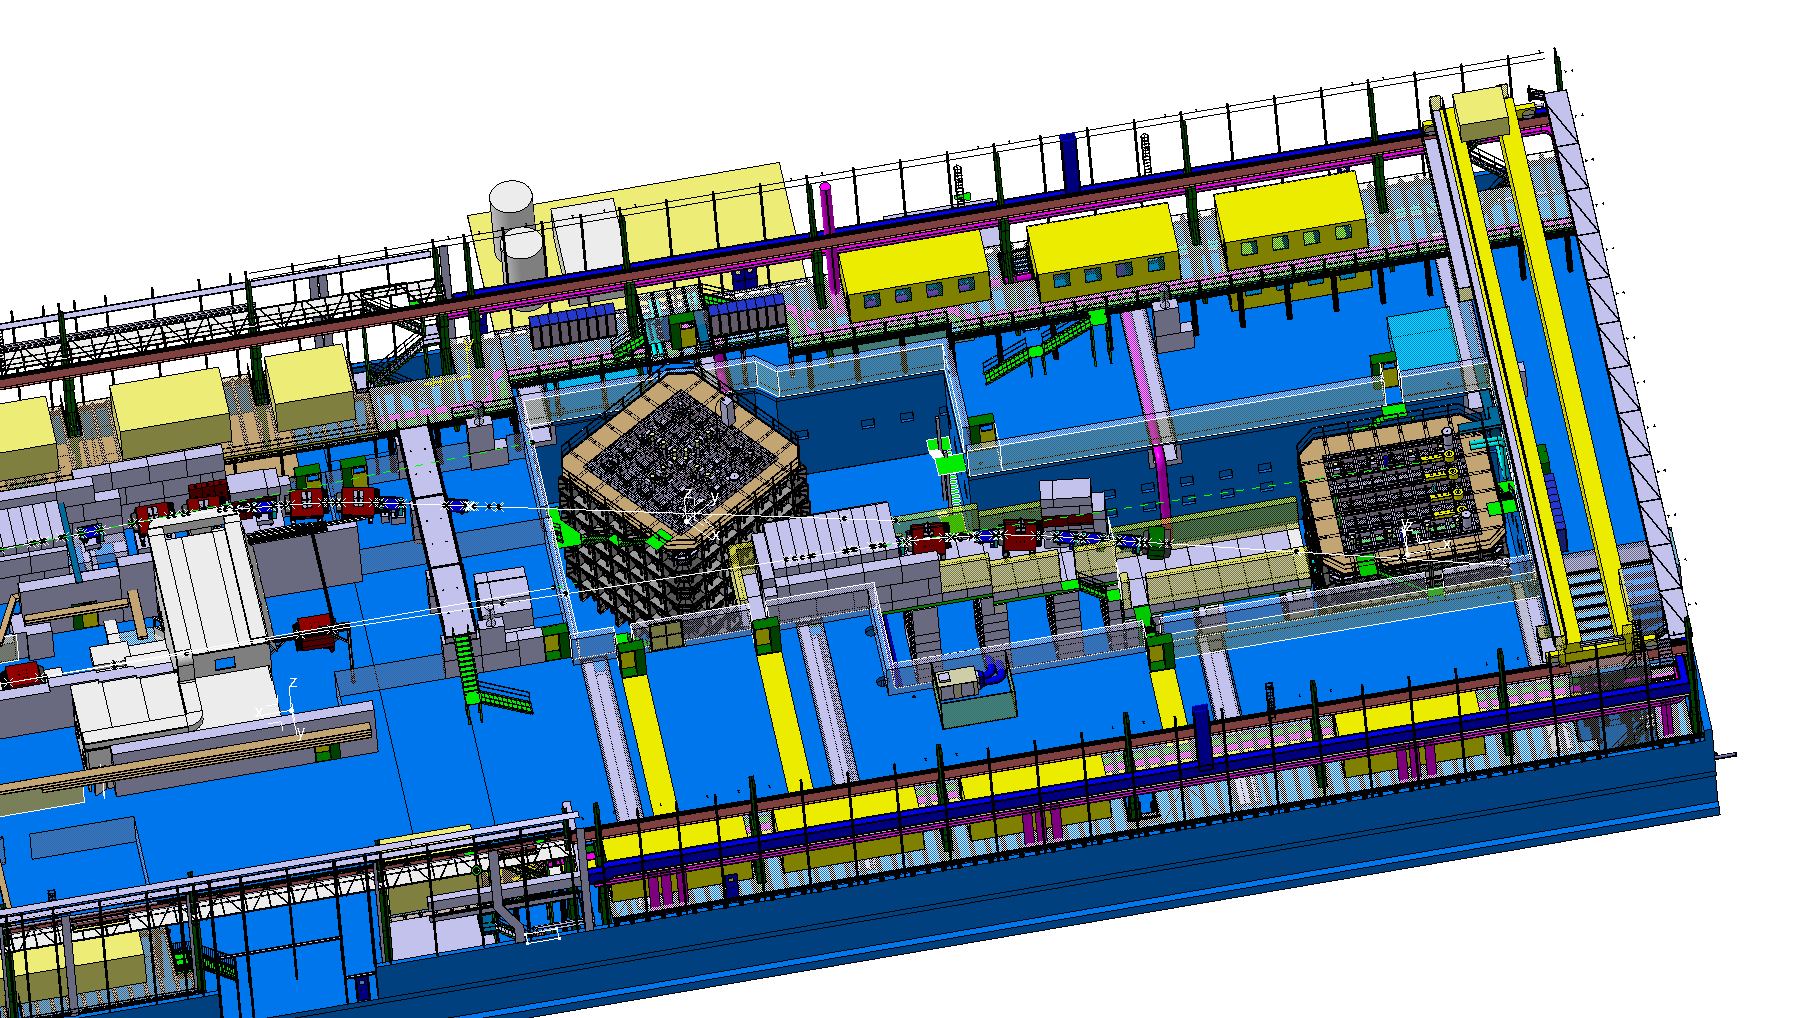
\includegraphics[width=1.0\textwidth]{figures/np02np04.png}
\caption{\label{fig:np02np04}Diagram of the layout of the CERN north area with
  location of the protoDUNE dual phase detector (center) and the single
  phase detector (right). The direction of the particle beam is from left to right.}
\end{figure}

\section{The protoDUNE-SP Data}
\subsection{Raw Data Parameters}
\label{sec:np04_data_rate}

The detector features the ``cold electronics'' design in which the amplifiers and digitizers
are placed within the cryostat and operate at cryogenic temperatures.
% Digital signals are fed to the Warm Interface Boards located outside of the cryostat on its top surface and then
% transmitted to the Data Acquisition System via a fiber optic line.
There are 15,360 channels read out at the 2\,MHz digitization frequency. The size of the data
read out from the detector in a single trigger cycle is approximately 230\,MB. At the nominal
trigger rate and lossless compression applied in the DAQ instantaneous data rate is about
1.5\,GB/s, and the sustained data rate to disk is 300\,MB/s.

\subsection{Data Flow and Distribution}
Principal elements of data transmission and storage in \pd are illustrated in Fig.\,\ref{fig:dataflow}.
Once the raw data are captured by the Data Acquisition System and written to the Online Buffer
located in the experimental hall  they are picked up by an instance of the \textit{Fermi FTS} system
\cite{sam,fts} which manages the transfer to the CERN distributed storage system (EOS).

EOS serves as the principal staging area from which the data get copied to tape storage and
are also transmitted to FNAL for offline processing by a separate instance of \textit{Fermi FTS}.
Importantly, EOS also serves to stage the input data for the prompt processing system and also to
store the outputs i.e. the various data products produced by DQM jobs. This design ensures
a large degree of independence of prompt processing and DQM from the DAQ and vice versa, but
it also introduces a latency due to the way data transfer from the Online Buffer operates. This latency is
of the scale of a few minutes and is considered acceptable in the context of DQM.

\begin{figure}[tb]
\centering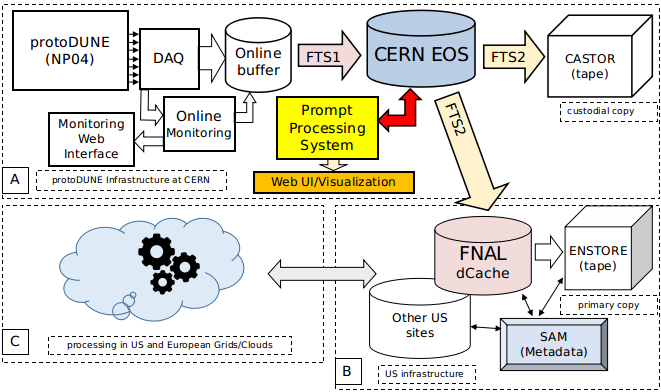
\includegraphics[width=0.9\textwidth]{figures/protoDUNE_data_flow_2018_v1.png}
\caption{\label{fig:dataflow}Diagram of the protoDUNE-SP data flow}
\end{figure}



\section{Data Quality Monitoring}
The protoDUNE-SP experiment will use an Online Monitoring system which obtains its input data directly
and in real time from the DAQ.
% Data Acquisition System.
 Its function is provide a very quick assessment of the general detector conditions
and to ascertain proper functioning of the readout chain. Online Monitoring characterized by low latency, high bandwidth
and limited CPU resources (located in the vicinity of the detector). This puts restrictions on what types of processing
can be usefully accomplished in this environment.
In order for more complex metrics to be calculated and actionable information to be provided to the experiment operators
(such as estimations of the Liquid Argon purity, signal characteristics after noise reduction, correlations of channel noise etc) 
the experiment will have a separate Data Quality Monitoring (DQM) system which complements the Online Monitoring.
This is similar to many High-Energy Physics experiments which implement ``express streams'' to perform
preliminary calculations on the data almost immediately after it leaves the DAQ. DQM is characterized by more relaxed
requiremens regarding latency of processing (which can take tens of minutes) and higher scalability, allowing
utilization of resources such the CERN Tier-0 computing facility.
%The \pd-SP DQM
It will include tasks such as
\begin{itemize}
\item Signal Processing (noise reduction, deconvolution) and basic Visualization in 2D projections
\item Liquid Argon purity monitoring using cosmic $\mu$ tracks
\item Basic monitoring of the Beam Instrumentation devices
\item Matching of beam particle tracks to signals deteected in the TPC
\end{itemize}


%For tables use syntax in table~\ref{tab-1}.
%\begin{table}
%\centering
%\caption{Please write your table caption here}
%\label{tab-1}       % Give a unique label
% For LaTeX tables you can use
%\begin{tabular}{lll}
%\hline
%first & second & third  \\\hline
%number & number & number \\
%number & number & number \\\hline
%\end{tabular}
% Or use
%\vspace*{5cm}  % with the correct table height
%\end{table}
%
% BibTeX or Biber users please use (the style is already called in the class, ensure that the "woc.bst" style is in your local directory)
% \bibliography{name or your bibliography database}
%
% Non-BibTeX users please use
%
\begin{thebibliography}{99}



\bibitem{cdrVol1}
R. Acciarri et al.
\emph{Long-Baseline Neutrino Facility (LBNF) and Deep Underground Neutrino Experiment (DUNE) Conceptual Design Report Volume 1: The LBNF and DUNE Projects}.\\ ~e-Print: arXiv:\textbf{1601.05471}
 %DUNE CDR Vol 1 -- The LBNF and DUNE Projects.~e-Print: arXiv:1601.05471
%\url{http://arxiv.org/abs/1601.05471}

\bibitem{cdrVol4}
R. Acciarri et al.
\emph{Long-Baseline Neutrino Facility (LBNF) and Deep Underground Neutrino Experiment (DUNE) Conceptual Design Report, Volume 4: The DUNE Detectors at LBNF}.\\~e-Print: arXiv:\textbf{1601.02984}
%\url{http://arxiv.org/abs/1601.02984}

\bibitem{eps} M.Potekhin et al. \emph{The protoDUNE-SP experiment and its prompt
processing system}. Proceedings of Science (EPS-HEP2017) 513

%\bibitem{uboone}
%B. Jones et al.  \emph{The Status of the MicroBooNE Experiment.~J. Phys.: Conf. Series.} Vol.\textbf{408}. IOP Publishing, 2013,
%doi:10.1088/1742-6596/408/1/012028

%\bibitem{castoreos}
% L. Mascetti et al. \emph{Disk storage at CERN.~J. Phys.: Conf. Series.} Vol.\textbf{664}. IOP Publishing, 2015,
%doi:10.1088/1742-6596/664/4/042035

\bibitem{sam}
R. A. Illingworth \emph{A data handling system for modern and future Fermilab experiments.~J. Phys.: Conf. Series.} Vol.\textbf{513}. IOP Publishing, 2014,
doi:10.1088/1742-6596/513/3/032045

\bibitem{fts}
A. Norman \emph{The Fermilab File Transfer System}.~e-Print: FNAL CD-DocDB-5412


%\bibitem{xrootd}
%L. Bauerdick et al. \emph{Using Xrootd to Federate Regional Storage.~J. Phys.: Conf. Series.} Vol.\textbf{396}. IOP Publishing, 2012,
%doi:10.1088/1742-6596/396/4/042009

\bibitem{panda}
T. Maeno et al. \emph{Overview of ATLAS PanDA Workload Management.~J. Phys.: Conf. Series.} Vol.\textbf{331}. IOP Publishing, 2011,
doi:10.1088/1742-6596/331/7/072024



\bibitem{dirac}
A. Casajus et al.  \emph{DIRAC Pilot Framework and the DIRAC
Workload Management System.~J. Phys.: Conf. Series.} Vol.\textbf{219}. IOP Publishing, 2010,
doi:10.1088/1742-6596/219/6/062049

\bibitem{django}
N. George \emph{Mastering Django: Core. The Complete Guide to Django 1.8 LTS}~ GNW Independent Publishing, ISBN: 099461683X



\end{thebibliography}


\end{document}

% end of file template.tex

%\begin{table}
%\begin{center}
%\caption{\label{table:np04_data_rate}
% protoDUNE-SP readout parameters}
%\ \\
%\begin{tabularx}{0.75\textwidth}{ X  >{\setlength{\hsize}{0.8\hsize}}r}
%\hline
%Detector Parameter & Target \\
%\hline
%TPC channel count & 15,360 \\
%Digitization frequency & 2\,MHz \\
%Nominal electron drift time & 2.2\,ms\\
%Nominal electron drift velocity & 1.6\,mm/$\mu$s\\
%Readout window & 5\,ms \\
%SPS spill time& 4.8\,s\\
%SPS cycle& 22.5\,s\\
%Nominal trigger rate & 25\,Hz \\
%Single readout size (per trigger) & 230.4\,MB \\
%Lossless compression factor (estimated) & 4 \\
%Instantaneous data rate (in-spill) & 1440\,MB/s \\
%Average data rate & 300\,MB/s \\
%Total data recorded (beam + cosmic) & 3\,PB\\
%Buffer to store 3 days worth of data & 300\,TB\\
%\hline
%\end{tabularx}
%\end{center}
%\end{table}

